\chapter{Materials and Methods}\label{chap:material_methods}
In this chapter, an overview of the dataset is initially presented in Section~\ref{sec:data}. This includes agronomic, geospatial, and meteorological data. Subsequently, in Section~\ref{sec:models}, in conjunction with the foundational information presented in the preceding Chapter~\ref{chap:background} and the data insights from Section~\ref{sec:data} of this chapter, we identify a suitable modeling strategy to address the research question. Following this, Sections~\ref{sec:mixed_to_gams} and \ref{sec:estimating_gams} offer a detailed examination of Mixed Models and Generalized Additive Models (GAM) as model fitting frameworks, along with our methodological contributions to estimating GAMs with tens of thousands of random effect factor levels.

\section{Data}\label{sec:data}
\subsection{Agronomic Data}\label{sec:agronomic_data}
We have access to historical milk sampling data from three major Swiss cow breeding associations \cite{swissherdbook2024}, \cite{braunvieh2024} and \cite{holsteinswitzerland2024}. The three associations have aims that are intimately linked to the breeding and promotion of particular cow breeds within Switzerland. Swissherdbook focuses mainly on Holstein, Simmental, and Swiss Fleckvieh. Holstein Switzerland is dedicated exclusively to Holstein and Red Holstein cattle. Meanwhile, Braunvieh Schweiz is centered around Braunvieh and Original Braunvieh cattle.

The data pool contains more information than test-day milk sample records. Along with these, the associations store breeding data, such as udder and other physical traits, insemination, and calving data. The \href{https://asr-ch.ch/images/content/Download-Ordner/Datenschnittstelle/RindviehCH_Interface-D.pdf}{data exchange standard} is defined by \cite{asr2024} and is maintained by \cite{qualitas2024}. This guarantees a common database format among the different breeding associations\footnote{In practice, some subtle differences between the different databases and schema versions exist.}.

Generally, breeding associations collect monthly test-day milk samples on dairy farms where the corresponding farmer participates in the breeding program. The exact sampling guidelines can be consulted in the milk inspector manual \citep{swissherdbook_2019}. Not all dairy farmers are part of a breeding association. Some conduct their own herd and breeding management on their farms and do not actively participate with their cows on the breeding market. However, the available data should be representative for Switzerland when considering the geospatial distribution of the data. The latter is further discussed in Section~\ref{sec:topological_data} and visualized in Figure~\ref{fig:dataset_sample_distribution}.

\paragraph{Data Processing}
For each of the three associations, the milk sample data is provided in a slightly different raw tabular database format. We write custom parsers on a best effort basis to process the individual datasets and merge the data from the three different providers into a single dataset. Table~\ref{table:k33_overview} summarizes a selection of available variables\footnote{We invite the reader to study further tables in the \cite{asr2024} specifications for follow-up projects.}. Note that each farm identifier can be linked with the corresponding farm metadata. This allows us to determine the farm location at the ZIP code level. The ZIP code associated with each sample is important for the matching process with the weather data. A finer granularity at the exact postal address level would be technically feasible but is not applied for data protection and privacy reasons.

\begin{table}[H]
    \centering
    \begin{tabular}{ll}
    \midrule
    \textbf{Milk Performance Variable} & \textbf{Description / Unit / Type} \\
    \midrule
    milk & Day milk yield [kg]\\
    fat & Fat [\%] \\
    protein & Crude protein [\%] \\
    ecm\_yield & Energy-corrected milk yield [kg]\\
    \midrule
    lactose & Lactose [\%] \\
    samplePersistence & Sample persistence [\%] \\
    somaticCellCount & Somatic cell count [x 1000/ml] \\
    milkUreaNitrogen & Milk urea nitrogen [mg/dl] \\
    citrate & Citrate [mg/dl]\\
    aceton & Aceton [mg/l] \\
    caseinMeasured & Casein [\%] \\
    acetonMmol & Aceton [mmol/l] \\
    acetonIr & Aceton IR (infrared spectroscopy) [mmol/l] \\
    bhbConcentration & BHB (beta-hydroxybutyrate) [mmol/l] \\
    \midrule
    \textbf{Metadata Variable} & \\
    \midrule
    animalId & Animal identification number [categorical]\\
    animalBreedCode & Animal breed code [categorical]\\
    farmIdLocationSample & Farm identification [categorical]\\
    calvingDate & Last calving date [date]\\
    lactationNumber & Lactation number [integer]\\
    sampleWeighingDate & Sample date [date]\\
    days\_in\_milk & sampleWeighingDate $-$ calvingDate [days]\\
    zip & ZIP matching the farm associated with farmIdLocationSample [categorical] \\
    \bottomrule
    \end{tabular}
    \caption{Subselection of \cite{asr2024} \href{https://asr-ch.ch/images/content/Download-Ordner/Datenschnittstelle/RindviehCH_Interface-D.pdf}{RindviehCH Interface Tables B01 and K33} Variables. Milk, fat and protein yield are the three primary variables of interest in our work. We manually define days\_in\_milk as the difference between \textit{sampleWeighingDate} and \textit{calvingDate}, and \textit{ecm\_yield} as a combination of \textit{milk}, \textit{fat} and \textit{protein} with \cite[Equation 9]{hall_invited_2023}.}
    \label{table:k33_overview}
\end{table}

\paragraph{Multi-Stage Data Cleaning Strategy}
We clean the raw data with the following multi-stage data cleaning strategy: First, we apply an interquartile range filter to milk, fat, and protein per breed and year. A sample is removed from the dataset if one of the three variables is an outlier. An outlier is defined as the value that lies below the lower bound $ Q_1 - 1.5 \times \text{IQR}$ or above the upper bound $ Q_3 + 1.5 \times \text{IQR} $, where $ Q_1 $ is the first quartile, $ Q_3 $ is the third quartile, and IQR is the range between the first and third quartiles, calculated as $\text{IQR} = Q_3 - Q_1 $.
Second, only those samples are considered where milk, fat, and protein measurements are all simultaneously available. Third, any samples linked to research farms, educational farm facilities, breeding associations, or research institutions are excluded as non-representative. Fourth, as there are some samples from outside the country, only Swiss farms, identifiable by their ZIP codes, are included. Fifth, samples where \textit{days\_in\_milk} exceed 600 days are discarded. Seventh, farms with less than 100 samples are excluded. Lastly, any animals contributing fewer than 5 samples are also eliminated.

\begin{table}[H]
\centering
\begin{tabular}{l l l l }
\textbf{Breed Code} & \textbf{Section} & \textbf{Mapped Code} & \textbf{Breed Name} \\
\hline
\hline
\cellcolor[HTML]{CDCDE7} RH & \cellcolor[HTML]{CDCDE7}Red Holstein & \cellcolor[HTML]{CDCDE7}HO & \cellcolor[HTML]{CDCDE7}\\
\cellcolor[HTML]{CDCDE7} HO & \cellcolor[HTML]{CDCDE7}Holstein & \cellcolor[HTML]{CDCDE7}HO & \cellcolor[HTML]{CDCDE7}Holstein \\
\cellcolor[HTML]{CDCDE7} RF & \cellcolor[HTML]{CDCDE7}Holstein & \cellcolor[HTML]{CDCDE7}HO & \cellcolor[HTML]{CDCDE7} \\
\hline
\cellcolor[HTML]{FFCCFF} SF & \cellcolor[HTML]{FFCCFF}Swiss Fleckvieh & \cellcolor[HTML]{FFCCFF}SF & \cellcolor[HTML]{FFCCFF}Swiss Fleckvieh \\
\hline
\cellcolor[HTML]{CCE5E5} BS & \cellcolor[HTML]{CCE5E5}Brown Swiss & \cellcolor[HTML]{CCE5E5}BS & \cellcolor[HTML]{CCE5E5}Brown Swiss \\
\hline
\cellcolor[HTML]{F1F1F1} 60 & \cellcolor[HTML]{F1F1F1}Simmental & \cellcolor[HTML]{F1F1F1}SI & \cellcolor[HTML]{F1F1F1}\\
\cellcolor[HTML]{F1F1F1} 70 & \cellcolor[HTML]{F1F1F1}Simmental & \cellcolor[HTML]{F1F1F1}SI & \cellcolor[HTML]{F1F1F1}Simmental\\
\cellcolor[HTML]{F1F1F1} SI & \cellcolor[HTML]{F1F1F1}Simmental & \cellcolor[HTML]{F1F1F1}SI & \cellcolor[HTML]{F1F1F1} \\
\hline
\cellcolor[HTML]{E2CDCD} OB & \cellcolor[HTML]{E2CDCD}Original Braunvieh & \cellcolor[HTML]{E2CDCD}OB & \cellcolor[HTML]{E2CDCD}Original Braunvieh \\
\hline
\cellcolor[HTML]{D0E6D0} JE & \cellcolor[HTML]{D0E6D0}Jersey & \cellcolor[HTML]{D0E6D0}JE & \cellcolor[HTML]{D0E6D0}Jersey \\
\hline
\end{tabular}
\caption{Breed codes and mapping according to \textit{Swissherdbook}.}
\label{table:breed_codes}
\end{table}


\paragraph{Breeds}
In the refined dataset, the \textit{animalBreedCode} variable encompasses 10 distinct breed codes. In accordance with the Swissherbook regulations \citep{swissherdbookregulations2022}, certain breed codes correspond to identical breeds. Breeding objectives are determined at the breed level; thus, codes 60, 70, and SI are unified under the same breeding goals. The same applies for the Holstein codes RH, HO and RF. A comprehensive overview is presented in Table~\ref{table:breed_codes}. This mapping is employed to streamline our dataset, enabling us to focus on 6 breeds in total: Holstein (HO), Jersey (JE), Brown Swiss (BS), Original Braunvieh (OB), Simmental (SI), and Swiss Fleckvieh (SF). Bloodline-specific breed information is available in the Swissherbook regulations. 

\begin{table}[H]
\centering
\renewcommand{\arraystretch}{1.2} % Adjust row height if needed
\begin{tabularx}{\textwidth}{>{\centering\arraybackslash}m{0.3cm}>{\centering\arraybackslash}m{2cm}>{\centering\arraybackslash}m{1.8cm}>{\centering\arraybackslash}X>{\centering\arraybackslash}X>{\centering\arraybackslash}X>{\centering\arraybackslash}X}
& \textbf{Breed} & \textbf{Purpose} & \textbf{Milk [kg/d]} & \textbf{Protein [\%]} & \textbf{Fat [\%]} & \textbf{ECM [kg/d]} \\
\hline
\hline
\rowcolor[HTML]{CDCDE7} $\circ$ & \textbf{Holstein} & Milk & 27.20 (±8.58) & 3.42 (±0.42) & 4.22 (±0.67) & 30.13 (±8.90) \\ \hline
\rowcolor[HTML]{FFCCFF} $\times$ & \textbf{Swiss Fleckvieh} & Milk/Meat & 22.45 (±7.51) & 3.46 (±0.42) & 4.27 (±0.69) & 25.02 (±7.88) \\ \hline
\rowcolor[HTML]{CCE5E5} $\bigtriangleup$ & \textbf{Brown Swiss} & Milk & 23.04 (±7.55) & 3.56 (±0.43) & 4.13 (±0.61) & 25.56 (±8.02) \\ \hline
\rowcolor[HTML]{F1F1F1} $\diamondsuit$ & \textbf{Simmental} & Milk/Meat & 19.39 (±6.50) & 3.44 (±0.37) & 4.04 (±0.60) & 21.14 (±6.89) \\ \hline
\rowcolor[HTML]{E2CDCD} $+$ & \textbf{Original Braunvieh} & Milk/Meat & 19.33 (±6.48) & 3.42 (±0.42) & 4.01 (±0.57) & 20.95 (±6.77) \\ \hline
\rowcolor[HTML]{D0E6D0} $\square$ & \textbf{Jersey} & Milk & 18.88 (±6.10) & 3.97 (±0.51) & 5.30 (±0.94) & 24.17 (±7.15) \\ \hline
\end{tabularx}
\caption{Annual milk performance average values for all breeds in the year 2023.}
\label{table:average_breed_performance_2023}
\end{table}

Table~\ref{table:average_breed_performance_2023} summarizes the national average dairy performance metrics for 2023. These values match the data reported by \cite{agrarbericht_2023} and \cite{sbv_2024}. In terms of milk yield, the Holstein breed is distinguished by its superior milk and ECM performance, whereas the Jersey breed is recognized for its elevated protein and fat yield. The latter characteristic is manifested in a comparatively greater enhancement in ECM-corrected performance relative to other breeds. These values also reflect the major characteristics of Swiss dairy farming presented in Chapter~\ref{chap:background}: The system is characterized by its familial orientation, limited scale, pasture-based approach, with a pronounced emphasis policy on sustainability and significant topological diversity. In particular, feeding practices are markedly different from those employed by high-yield dairy enterprises in regions such as the United States. 

\begin{table}[H]
\centering
\renewcommand{\arraystretch}{1.2}
\begin{tabularx}{\textwidth}{>{\centering\arraybackslash}m{0.3cm}>{\raggedright\arraybackslash}m{3cm}>{\centering\arraybackslash}X>{\centering\arraybackslash}X>{\centering\arraybackslash}X>{\centering\arraybackslash}X}
 & \textbf{Breed} & \textbf{\# Samples} & \textbf{\# Farms} & \textbf{\# Animals} & \textbf{Timespan} \\
\hline
\hline
\rowcolor[HTML]{CDCDE7} $\circ$ & \textbf{Holstein} & 27'536'089 & 24'963 & 971'198 & 1985-2023 \\ \hline
\rowcolor[HTML]{FFCCFF} $\times$ & \textbf{Swiss Fleckvieh} & 31'484'784 & 27'392 & 1'038'291 & 1984-2023 \\ \hline
\rowcolor[HTML]{CCE5E5} $\bigtriangleup$ & \textbf{Brown Swiss} & 56'695'579 & 26'585 & 1'719'156 & 1982-2023 \\ \hline
\rowcolor[HTML]{F1F1F1} $\diamondsuit$ & \textbf{Simmental} & 8'731'867 & 19'411 & 299'698 & 1984-2023 \\ \hline
\rowcolor[HTML]{E2CDCD} $+$ & \textbf{Original Braunvieh} & 4'996'060 & 18'613 & 149'478 & 1982-2023 \\ \hline
\rowcolor[HTML]{D0E6D0} $\square$ & \textbf{Jersey} & 734'685 & 4'302 & 23'675 & 1998-2023 \\ \hline
 & Total & 130'179'064 & 46'975 & 4'201'494 & 1982-2023 \\ \hline
\end{tabularx}
\caption{Dataset statistics: the cleaned dataset contains over 130 million samples from 4.2 million animals distributed on almost 47 thousand farms between 1982 and 2023.}
\label{table:dataset_statistics}
\end{table}

In Table~\ref{table:dataset_statistics}, we summarize the sample distributions across breeds, farms and animals. The over 130~million samples are not equally distributed among the breeds. Brown Swiss is leading with over 56 million samples, followed by Swiss Fleckvieh with over 31 million samples. Holstein\footnote{According to Holstein Switzerland, some data is irrecoverably lost.} has about 27~million samples. Simmental and Original Braunvieh follow with 8.7~million and almost 5~million samples. For the Jersey breed over 730'000 samples are available. On average, 30~samples per cow are available. Along with the number of samples, we report the number of farms and animals as well as the time range covered by the samples available. The overall dataset has samples from more than 4~million cows spanning a time period of 42 years. The ratios between the number of samples, farms and animals reveal different farm structures for the different breeds. Therefore, data subsampling strategies, if required, need to be applied with care. Moreover, farms can host multiple dairy cow breeds.


\begin{figure}[H]
    \centering
    % First figure
    \begin{subfigure}[b]{\textwidth}
        \centering
        
\includegraphics[width=\textwidth]{thesis/figures/dataset/dataset_structure_1.png}
    \end{subfigure}
    \begin{subfigure}[b]{\textwidth}
        \centering
        
\includegraphics[width=\textwidth]{thesis/figures/dataset/dataset_structure_2.png}
    \end{subfigure}
    
    \caption{Structure of our data: sparsity and dynamics. Farms enter and exit. Animals enter and exit. Animals move. The sampling frequency is irregular.}
    \label{fig:dataset_structure_sparsity_dynamics}
\end{figure}

\paragraph{Data Structure: Sparsity and Dynamics}
Figure~\ref{fig:dataset_structure_sparsity_dynamics} depicts the sparse structure and intrinsic dynamics of the dataset. We describe subfigures top down and from left to right. The initial subfigure presents the distribution of samples across individual farms, indicating that the majority possess several thousand samples. The subsequent distribution demonstrates the longitudinal data availability across years for the farms, highlighting that some farms intermittently enter or exit the panel, while others continuously contribute samples over nearly four decades. The third figure underscores the spatial dynamics of livestock. We observe that most cattle are kept on the same farm. However, some cattle relocate, a phenomenon attributable to seasonal pasture changes as well as commercial activities such as breeding exchanges. The fourth figure elucidates the distribution of the number of samples collected over an animal's lifespan or its tenure in the panel. The subsequent subfigure indicates that the majority of animals are sampled over a period ranging from 2 to 5 years. Consequently, similar to farms, animals enter and exit the panel. The final figure reveals that each year, only a limited number of samples are available from the animals.

\vspace*{\baselineskip}
In conclusion, the dataset reflects actual agricultural practices and farm structures in Switzerland, rather than being designed for controlled experimental studies measuring biological responses of dairy cows. The data is primarily collected to monitor long-term breeding progress. Hence, the dataset is notably sparse, in stark contrast to experimental research, where data collection from farms and cows occurs with greater frequency and regularity. Addressing our research question necessitates a diverse set of THI data points. When breeding associations conduct sampling on a farm, they sample all cows on the test day. Consequently, on average, there are 7 weather data points recorded per cow, farm, and year. Therefore, a representative sample covering a broad spectrum of THI data points requires data from at least hundreds of farms and thousands of animals.

\begin{figure}[H]
\centering
\includegraphics[width=0.8\textwidth]{thesis/figures/dataset/dataset_structure_3.png}
\caption{Structure of our data: time and seasonality. The figure illustrates the average daily milk production per cow in Switzerland for the years 1990, 2000, 2010, and 2020.}
\label{fig:dataset_structure_time_seasonality}
\end{figure}

\paragraph{Data Structure: Time and Seasonality}
The average milk yield per cow shows a continuous annual increase. Figure~\ref{fig:dataset_structure_time_seasonality} illustrates the average daily milk yield of cows recorded on the corresponding days in the years 1990, 2000, 2010, and 2020 in Switzerland across all breeds. There is a notable increase in daily milk production over the years attributable to advancements in breeding. Additionally, seasonal fluctuations are apparent throughout each year. The minor spikes observed are a consequence of the sampling strategies employed by breeding associations, as farms are sampled sequentially rather than simultaneously. The peak of lactation occurs approximately in April and May, influenced by farm management practices. Seasonal calving during winter months results in lactation peaks during these months, supported by the availability of high-quality grasslands in the spring season. Consequently, the reduced milk yield observed during the summer months can be attributed not solely to heat stress, but also to the biological cycle, geospatial factors, farm management practices, and the availability of grassland. These long-term and seasonal factors must be appropriately modeled to accurately assess the impact of the THI on dairy performance.


\begin{figure}[ht]
    \centering
    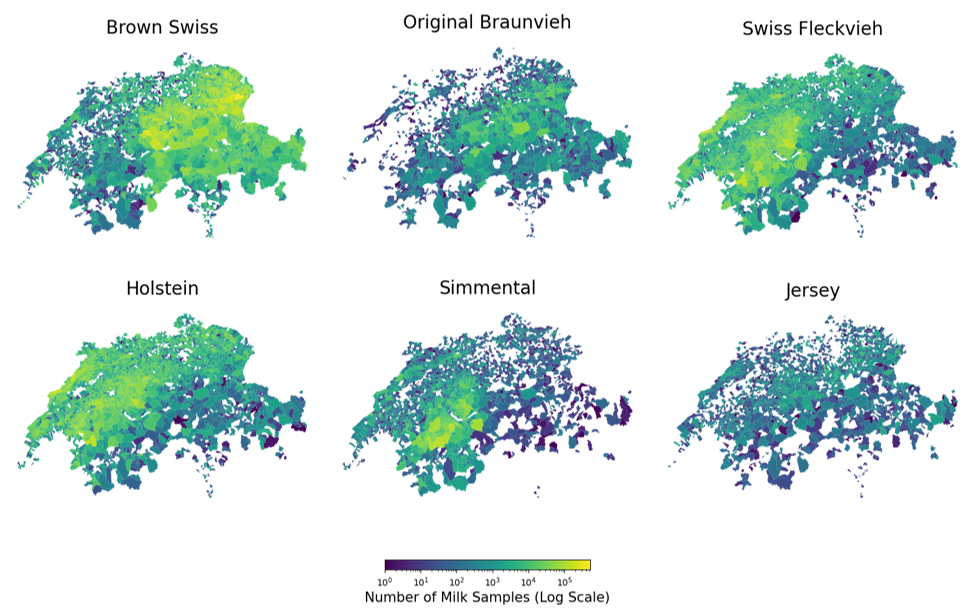
\includegraphics[width=\textwidth]{thesis/figures/dataset/sample_distribution.png}
    \caption{Sample distribution for each dairy cow breed.}
    \label{fig:dataset_sample_distribution}
\end{figure}

\subsection{Geospatial Data}\label{sec:topological_data}
The milk data described in Section~\ref{sec:agronomic_data} is provided with anonymized farm metadata with associated ZIP codes. In Switzerland, each ZIP code can be mapped to a locality. A locality is a geographically defined area designated by an unambiguous place name and unique ZIP code. The ZIP belongs to one or more political municipalities. The latter have a unique BFS\footnote{Bundesamt für Statisik - Federal Statistics Office} number assigned by the Swiss Federal Statistics Office. Since the locality distribution is more fine-granular than the political municipalities, we map each farm to the closest geographical locality center. We count a total of $3194$ localities. The geospatial data and altitude raster grids are retrieved from \cite{swisstopo_2024, swisstopo_2024_dhm25}. By matching the locality data with the milk samples ZIP codes, we delineate the geospatial distributions of samples per breed, as illustrated in Figure~\ref{fig:dataset_sample_distribution}. The Simmental and Swiss Fleckvieh populations are predominantly located in the Bernese Alps\footnote{We can also refer them as the "typical" mountain cow breeds}, whereas the Holstein breed is primarily found in Western Switzerland. In contrast, the Brown Swiss and Original Braunvieh breeds are more prevalent in eastern Switzerland. The Jersey breed, however, demonstrates a more scattered geographical distribution.



\subsection{Hydroclimatic Data}\label{sec:meteo_data}
Meteorological variables such as daily mean, minimum and maximum temperatures in [°C], precipitation [mm] and relative sunshine duration [\%] are available as a gridded dataset from \cite{ethz_2024_meteoswiss} with a 1[km]x1[km] resolution. We allocate each ZIP code locality center to the nearest point within the gridded dataset. The relative humidity is not available in gridded form. Nonetheless, the THI metric requires the relative humidity measure. \cite{meteoschweiz_2024_idaweb} offers daily mean, minimum and maximum relative humidity for some weather stations. We follow \cite{bucheli_temperature_2022} and map available height corrected stations to the closest height corrected locality centers with the following distance function: 
\begin{equation}\label{eq:station_distance_function}
    d_{s,c} = \sqrt{(\text{lat}_s - \text{lat}_c)^2 + (\text{long}_s - \text{lat}_c)^2 + \left(\psi \cdot (\text{alt}_s - \text{elevation}_c)\right)^2}.
\end{equation}
The height correction is integrated in $d_{s,c}$ as a factor $\psi=100$. This correction is applied because relative humidity is more likely to vary with elevation changes than with horizontal movements. The temperature varies with altitude and changes the saturation capacity.

\begin{figure}[htbp]
    \centering
    \begin{subfigure}[b]{0.45\textwidth}
        \centering
        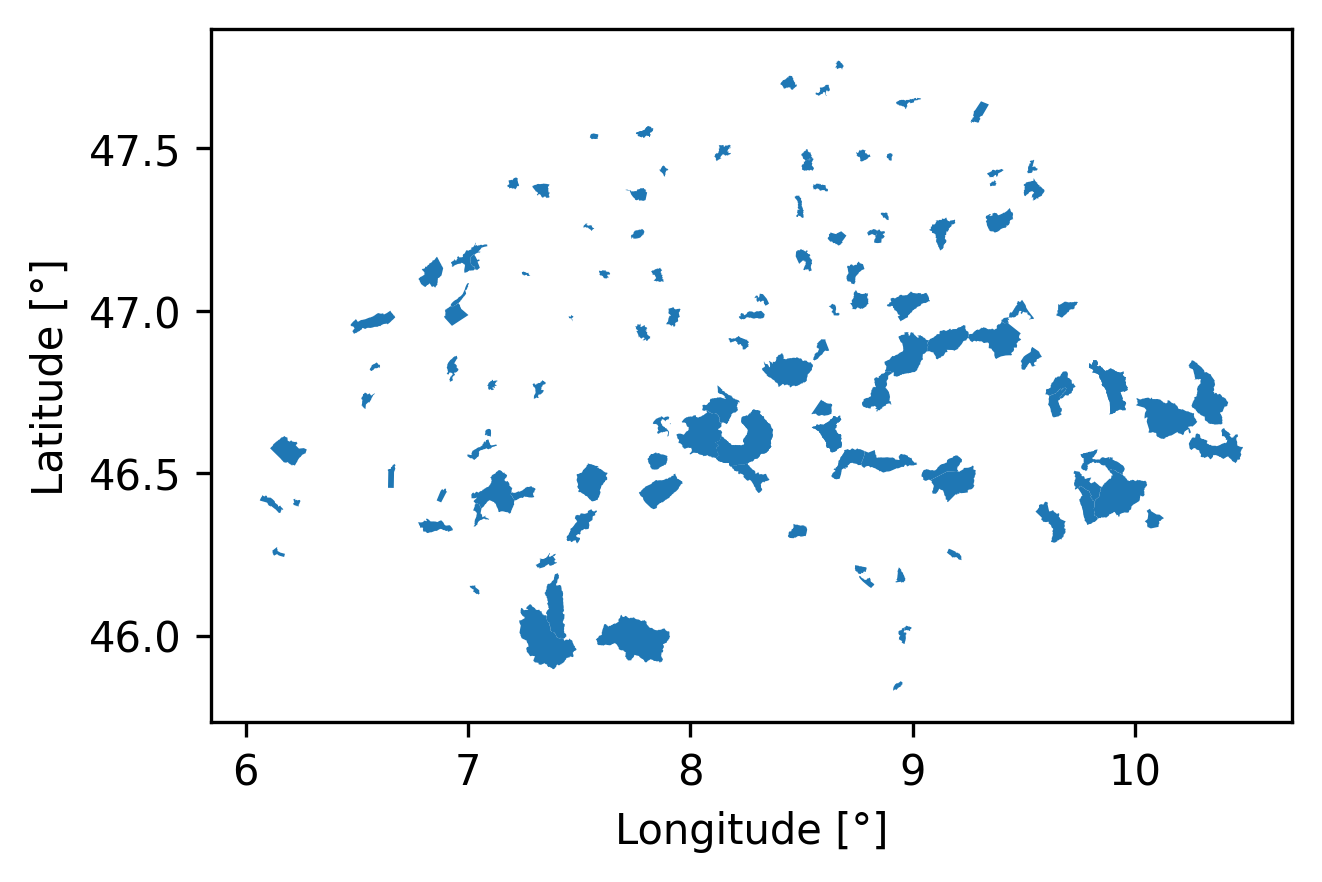
\includegraphics[width=\textwidth]{thesis/figures/weather_stations_1982.png}
        \caption{1982 - 159 Stations}
        \label{fig:weather_stations_1982}
    \end{subfigure}
    \hfill
    \begin{subfigure}[b]{0.45\textwidth}
        \centering
        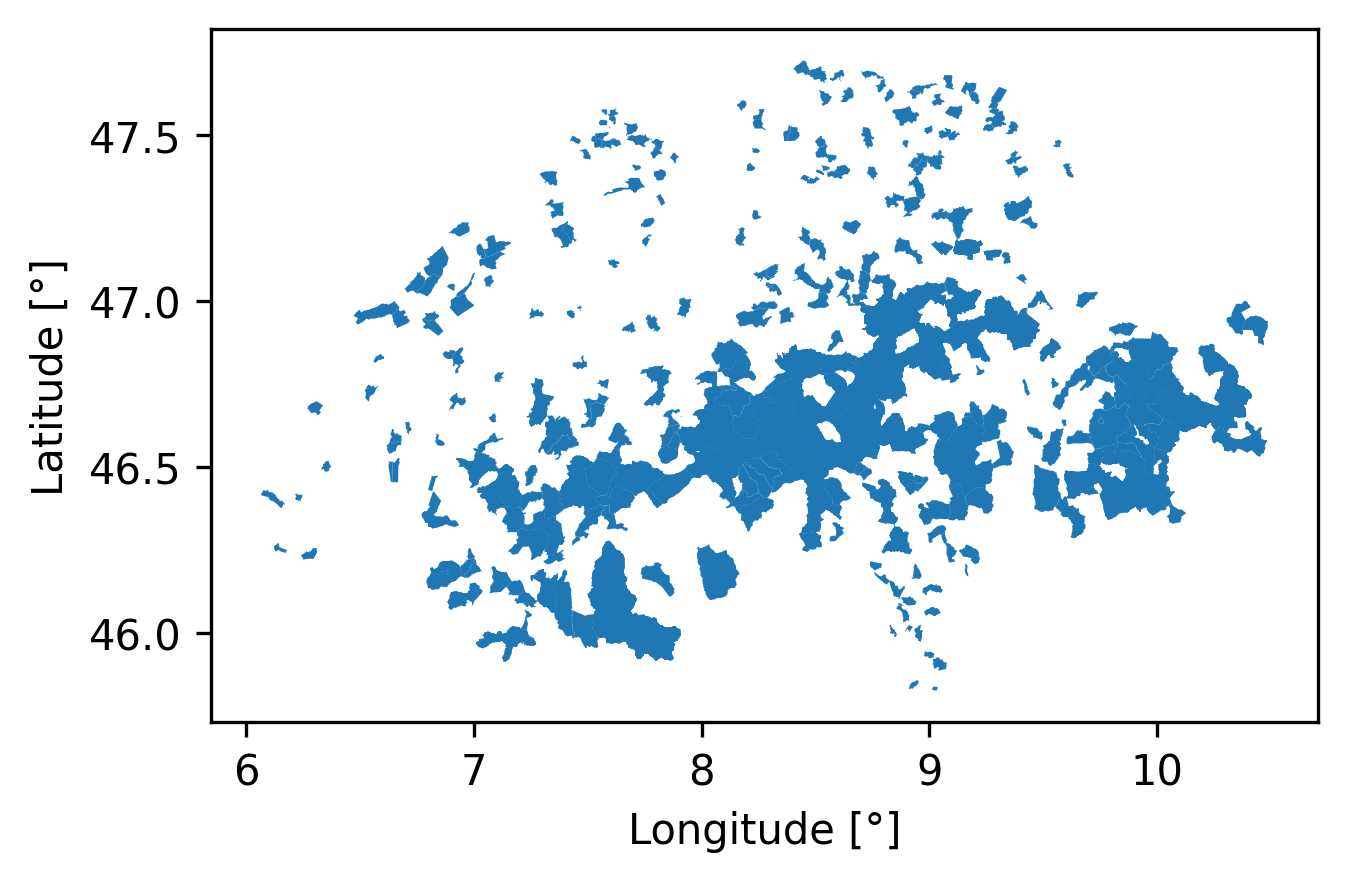
\includegraphics[width=\textwidth]{thesis/figures/weather_stations_2023.png}
        \caption{2023 - 540 Stations}
        \label{fig:weather_stations_2023}
    \end{subfigure}
    \caption{Geographical weather station distribution with available relative humidity data.}
    \label{fig:weather_stations}
\end{figure}

We retrieve all daily mean, maximum and minimum relative humidity data available from the MeteoSuisse portal from 1982 until the end of 2023. The following requirements for a station to be considered: First, the station must not have more than 500 missing samples during its lifetime. We treat a station as long as it exists as a fixed measurement point and do not control for technical changes such as hardware upgrades, which increases risk of instrumentation bias. Under these constraints, $159$ stations are available in 1982 and $540$ by the end of 2023. Figure~\ref{fig:weather_stations} shows the weather station distribution in these two years. The station concentration is increasing more in the alpine regions than in the Swiss plateau. During our study period from 1982-2024, all major regions in Switzerland are equipped with weather stations, and they increase in density over time.


\section{Models}\label{sec:models}
Informed by modeling elements derived from prior research, background information regarding dairy farming in Switzerland, biological aspects, and the organization of our data, we establish an empirical strategy. Then, we derive two model classes: single-breed models which are estimated with data for each breed-separately, and multi-breed models which are estimated with data from all breeds together. Single-breed models have lower complexity and are easier to estimate. However, this comes with statistical challenges for model comparison. A multi-breed model that explicitly models the breed aspects introduces more complexity and might be harder to estimate. However, in certain circumstances, this is more appropriate for valid statistical comparisons between breeds.

\subsection{Empirical Strategy}\label{sec:empirical_strategy}
Our goal is to estimate the average effect of THI on cow-level dairy production performance variables while controlling for breed, animal-physiological aspects, and other environmental effects such as farm management practices, regulatory changes, and breeding progress. Hence, we need an additive statistical approach to separate the THI effect from these other factors. This requirement leads us to a model with the following structure:

\begin{equation}\label{eq:empirical_strategy}
    \textit{Variable of Interest} = \textit{Weather} + \textit{Controls} + \textit{Unobserved Heterogeneity} + \textit{Error}.
\end{equation}

The \textit{variables of interest} are the daily milk yield and daily ECM yield. To estimate the average effect of weather, we need to model the THI as a component. We know from prior research that the effect of THI on milk and milk component performance is non-linear. In our models, we will use the three-day mean THI. This is the average THI value from the milk sample date $t$, $t-1$ and $t-2$: 

\begin{equation}
    \textit{3 Day Mean THI} = \frac{THI_t + THI_{t-1} + THI_{t-2}}{3},
\end{equation}
where $t$ is the reported milk sample date and 
\begin{equation}
    \text{THI}_t = (1.8 \times \text{T}_t) + 32 - \left[ (0.55 - 0.0055 \times \text{RH}_t) \times (1.8 \times \text{T}_t - 26) \right].
\end{equation}
 $T_t$ and $RH_t$ are the mean temperature and mean relative humidity of day $t$.

We opt for the three-day THI mean based on several considerations: Firstly, when a farm is sampled, cows are sampled in the morning and in the evening. These samples may either be collected on the same calendar day or across two consecutive days when the samples are taken in the evening and the morning of the following day. In the latter case, the sample date is recorded as the morning of the subsequent day; this is irrespective of the first sample being taken the day prior. The specific sequence of sampling for each set is not discernible within the dataset. Although such details are inconsequential for practical breeding operations, they become critical when aligning milk sample data with meteorological information. Consequently, it is imperative to account for weather conditions on the sampling day as well as one day prior. Secondly, we incorporate an additional preceding day to address the lagged effect of the THI on dairy cows. Currently, there is no standardized consensus on the number of lag days to be considered. However, we have aligned our methodology with the approach delineated in \cite{bryant_quantifying_2007}.

The model needs to \textit{control} for the non-linear lactation curve of the cow. Right after calving,  the milk performance increases until it reaches a peak point before it drops again until the next dry period starts. A viable proxy for this purpose is days in milk (DIM). Moreover, dairy performance also depends on the the parity - we make a binary distinction between primi- and multiparous cows. Primiparous cows have not developed their full biological potential and have a lower milk performance than multiparous cows. Moreover, we also need to control for the within-year seasonality, geospatial differences, and long-term effects such as breeding progress or regulatory changes. These aspects are motivated by the analysis of effects observed in Figure~\ref{fig:dataset_structure_time_seasonality}.

The specific characteristics of the farm location, including the barn infrastructure, the topographical features and the management strategies, cannot be explicitly measured. We assume farmers constantly adapt and change their best practices. Similarly, the fundamental performance attributed to the genetic and phenotypic attributes of individual cows cannot be directly observed. It is imperative to account for this latent heterogeneity.

\subsection{Single Breed Model}\label{sec:single_breed_model}
We first introduce a single breed model before expanding it in the next section.
Let $y_{ijkt}$ be a dairy performance variable of a sample of animal~$i$, at the farm location~$j$, at farm $k$ and at the sampling date~$t$. Equation~\ref{eq:single_breed_model_extended} defines an additive mixed model to estimate the average effect of THI on milk performance variables. The coefficient $\beta_0$ is the intercept which represents the mean performance of the given breed data, excluding all other factors included in the model. $\mathbb{I}(\text{Primiparous}_i)$ is the indicator variable whether the current cow $i$ is primi- or multiparous. $\textit{THI}_{kt}$ is the three-day mean THI at the farm location $k$ at the sampling date $t$. THI is modelled as a separate non-linear function $f_{1,1}$ and $f_{1,2}$ for primi-and multiparous cows. $\textit{DIM}_{it}$ is the days milk of the cow $i$ sampled on day $t$. Following the same analogy as for THI, DIM is also modelled separately as a non-linear function $f_{2,1}$ and $f_{2,2}$ for primi- and multiparous cows. $\beta_1$ is the fixed effect coefficient for being primiparous compared to multiparous. $\mathbb{I}(\text{Year}_t = m)$ is a variable indicating whether the sampling date $t$ falls in the year $m$, where $\mathcal{M}$ is the set of years covered by the samples included. $\beta_{2,m}$ is the effect of year $m$ compared to the reference year. $\iota_{kt}$ is the random intercept for $ZIP$ of farm $k$ and month of the sample date $t$. This random effect models the annual seasonality accounting for geospatial differences; due to the topological heterogeneity of Switzerland, timing and farming practices might vary. For example, in high-altitude regions the grazing season might start later than in the Swiss Plateau. Another aspect which is covered by this random intercept are spatial spillovers. Neighbouring farmers might apply similar practices simply due to geospatial constraints but also due to networking effects \citep{young1959neighborhood}. The factor levels for this random intercept are created with a ZIP code - month interaction term. The ZIP code is a natural choice originating from our farm-ZIP code matching introduced in Section~\ref{sec:data} and the monthly granularity is justified by the monthly sampling frequency by the breeding associations\footnote{Both of these hyperparameters are somewhat arbitrary and could be optimized in a model selection process.}. $\phi_{k}$ is the random intercept for the location of farm $k$. First, since different farms have unique characteristics such as soil, land or barn we capture the variability between farms. Moreover, Figure~\ref{fig:dataset_structure_sparsity_dynamics} shows us the hierarchical structure of the data. Grouping within entities such as farms needs to be taken into account in the model. With our data we cover very long periods of time. Farmers constantly adopt and change their practices over time. Some of the long-term national average aspects are captured by the $\textit{Year}$ fixed effect. The constant individual adaptation by each farmer is not explicitly modelled. Consequently, the effects \( f(THI) \) and \( f(DIM) \) are, at least in part, implicitly reflective of adaptive changes. Additionally, each individual cow $i$ is incorporated as a random intercept $\alpha$ to account for repeated sampling per cow and distinctive animal characteristics. The residual error term is denoted by $\epsilon_{ijkt}$.

\begin{defi}Single Breed Model - Extended Notation
\begin{equation}\label{eq:single_breed_model_extended}
    \begin{aligned}
        y_{ijkt} = & \ \beta_0 \\
        & + f_{1,1}(\text{THI}_{kt}) \cdot \mathbb{I}(\text{Primiparous}_i) \\
        & + f_{1,2}(\text{THI}_{kt}) \cdot (1 - \mathbb{I}(\text{Primiparous}_i)) \\
        & + f_{2,1}(\text{DIM}_{it}) \cdot \mathbb{I}(\text{Primiparous}_i) \\
        & + f_{2,2}(\text{DIM}_{it}) \cdot (1 - \mathbb{I}(\text{Primiparous}_i)) \\
        & + \beta_1 \cdot \mathbb{I}(\text{Primiparous}_i) \\
        & + \sum_{m \ in \mathcal{M}} \beta_{2m} \cdot \mathbb{I}(\text{Year}_t = m) \\
        & + \iota_{kt} \\
        & + \phi_k \\
        & + \alpha_i \\ 
        & + \epsilon_{ijkt} 
    \end{aligned}
\end{equation}
\end{defi}

In Equation~\ref{eq:single_breed_model} we provide a simplified notation for the model introduced in Equation~\ref{eq:single_breed_model_extended} solely focusing on the covariates and not their coefficients.

\begin{defi} Single Breed Model - Simplified Notation
\begin{equation}\label{eq:single_breed_model}
y = \mu + f(\text{THI}) \cdot \text{P} + f(\text{DIM}) \cdot \text{P} + \text{P} + \text{Y} + \iota + \phi + \alpha + \epsilon
\end{equation}
\end{defi}
The variable $y$ denotes the dependent dairy performance variable. The parameter $\mu$ serves as the overall intercept of the model. The function $f(\text{THI})$ is a non-linear function relating to the THI. Likewise, $f(\text{DIM})$ is a non-linear function that models the lactation curve. The variable $\text{P}$ signifies parity, representing a binary distinction between primiparous and multiparous cows. The term $\text{Y}$ symbolizes the year as a categorical variable, capturing potential year-to-year variations. The random intercept $\iota$ accounts for variation linked to the zip code by month, reflecting geographic and seasonality. The random intercept $\phi$ pertains to the farm location, managing variability across different farms and sampling sites. The random intercept $\alpha$ addresses the variability among individual cows. Lastly, $\epsilon$ denotes the residual error term of the model.

\subsection{Mutli-Breed Model}\label{sec:multi_breed_model}
Our hypothesis posits varying effects of THI on dairy performance across different breeds. Consequently, our aim is to determine whether there are statistically significant heterogeneous treatment effects. The treatment under consideration is the exposure of cows to weather (THI), while the heterogeneity arises from the various dairy cow breeds. Dividing the data based on breed and estimating separate models for each breed is appealing for reducing modeling complexity; however, challenges may arise if not all covariates are interacted with breed in a multi-breed model, since statistical significance is contingent upon all covariates \citep{le_interaction_term_2020}. With biological reasoning, it is justifiable to consider separate intercepts as well as interaction terms involving f(THI), f(DIM), parity, and year. The interaction of random effects for seasonality and location by breed requires further investigation. The central question pertains to whether we should assume a common biological response across breeds with respect to location and farm. Given that each cow is associated with a single breed, it should not matter whether the random intercept for cow $\alpha_i$ is interacted by breed or not. An example multi-breed models following the arguments above is

\begin{defi}
\begin{equation}\label{eq:multi_breed_model_extended}
    \begin{aligned}
        y_{ijkt} = & \ \sum_{b \in \mathcal{B}} \beta_{0,b} \cdot \mathbb{I}(B_i = b) \\
        & + \sum_{b \in \mathcal{B}} \left[ f_{1,1,b}(\text{THI}_{kt}) \cdot \mathbb{I}(\text{Primiparous}_i) \cdot \mathbb{I}(B_i = b) \right] \\
        & + \sum_{b \in \mathcal{B}} \left[ f_{1,2,b}(\text{THI}_{kt}) \cdot (1 - \mathbb{I}(\text{Primiparous}_i)) \cdot \mathbb{I}(B_i = b) \right] \\
        & + \sum_{b \in \mathcal{B}} \left[ f_{2,1,b}(\text{DIM}_{it}) \cdot \mathbb{I}(\text{Primiparous}_i) \cdot \mathbb{I}(B_i = b) \right] \\
        & + \sum_{b \in \mathcal{B}} \left[ f_{2,2,b}(\text{DIM}_{it}) \cdot (1 - \mathbb{I}(\text{Primiparous}_i)) \cdot \mathbb{I}(B_i = b) \right] \\
        & + \sum_{b \in \mathcal{B}} \left[ \beta_{1,b} \cdot \mathbb{I}(\text{Primiparous}_i) \cdot \mathbb{I}(B_i = b) \right] \\
        & + \sum_{m \in \mathcal{M}} \beta_{2m} \cdot \mathbb{I}(\text{Year}_t = m) \\
        & + \iota_{kt} \\
        & + \phi_k \\
        & + \alpha_i \\
        & + \epsilon_{ijkt},
    \end{aligned}
\end{equation}
\end{defi}

where $\mathcal{B}$ is the set of available breeds and $B_i$ a binary indicator for breed.

\subsection{Model Estimation Strategy}\label{sec:estimation_strategy}
Given the presence of repeated unbalanced measurements for cows and farms as illustrated in Table~\ref{table:dataset_statistics} and Figure~\ref{fig:dataset_structure_sparsity_dynamics}, the application of mixed models with maximum likelihood estimation is deemed appropriate for our model estimation \cite[page 61 and 74]{wood_generalized_2017}. Various methodologies exist to model the non-linear components $f$, such as binning, piecewise regression (broken stick), or splines. The contemporary approach for estimating non-linearities is through smooth terms, which can be implemented within a Generalized Additive Model framework \citep[Chapter 5 and 6]{wood_generalized_2017}. Smooth terms, being splines with penalized coefficients, facilitate a more accurate representation of the data. Consequently, we characterize our nonlinear functions $f$ as smooth terms. The components of our models are a combination of smooth terms, fixed effects, and random effects, thereby constituting Generalized Additive Mixed Models \citep[page 288]{wood_generalized_2017}. To address our research question with an estimated model, we numerically derive the turning points in the smooth terms $f$. We use \textit{mgcv} \citep{mgcv1, mgcv2, mgcv4, wood_generalized_2017, wood_gamm4_2020} for estimation and \textit{gratia} \citep{gratia} for the turning point search. This purely data-driven approach for inflection point determination is a considerable improvement compared to previous works which make preliminary assumptions about the non-linearities. Implementation details and library modifications required for our data are discussed in the following sections.


\section{From Linear Mixed Models to Generalized Additive Mixed Models}\label{sec:mixed_to_gams}
To link our model definitions in Section~\ref{sec:models} with the GAMM framework, we provide the basics around mixed models, GAMs and GAMMs and explain how they are linked. Understanding the relationship between these three frameworks is vital for a successful and computationally efficient estimation of Equation~\ref{eq:single_breed_model_extended} and Equation~\ref{eq:multi_breed_model_extended}.

\subsection{Generalized Linear Mixed Models}\label{sec:glmm}
We use the definitions from \citet{wood_generalized_2017} and \citet{bates_fitting_2015} to introduce mixed models. Let $\bm{y} \in \mathbb{R}^n$ be the response data of $n$ samples from a random variable $\mathcal{Y}$ belonging to the exponential family. Let $g(\mu_i)=\mathbf{X}_i \bm{\beta}$, where $\mu_i \equiv \mathbb{E}(Y_i)$, $g$ is the link function, $\mathbf{X}_i$ is the $i$-th row of the model matrix $\mathbf{X} \in \mathbb{R}^{n \times p}$ and $\bm{\beta} \in \mathbb{R}^p$ the vector of the  $p$ fixed effect parameters. The response variable samples $y_i$ are assumed to be independent and have a distribution that belongs to the exponential family. Let $\mathbf{Z}_i$ be the $i$-th row of the random effect model matrix $\mathbf{Z} \in \mathbb{R}^{n \times q}$ , and let $\bm{b} \in \mathbb{R}^{q}$ be the q-dimensional random vector from a random variable $\mathcal{B}\sim \mathcal N(\bm{0},\bm{\psi_{\theta}})$ containing random effects with zero expected value and covariance matrix $\bm{\psi_{\theta}} \in \mathbb{R}^{q \times q}$ with unknown parameters~$\bm{\theta}$. Let $\mathbf{\Lambda_{\theta}} \in \mathbb{R}^{n \times n}$ be the residual covariance matrix to model the residual autocorrelation. We assume that the residuals are distributed independently and identically. Hence, $\bm{\Lambda{\theta}} = \mathbf{I}\sigma^2$. This simplification comes with computational advantages, but also with modelling drawbacks regarding spatial autocorrelation in our data.
\\
\\
For the Gaussian case, a Linear Mixed Model (LMM) is defined as
\begin{defi}Linear Mixed Model
    \begin{equation}\label{eq:lmm}
    \mathbf{y} = \mathbf{X}\bm{\beta} + \mathbf{Z}\bm{b} + \bm{\epsilon}, \quad \bm{b}\sim N(\bm{0}, \bm{\psi_{\theta}}), \quad \bm{\epsilon} \sim \mathcal(\bm{0}, \bm{\Lambda_{\theta}}) = N(\bm{0},\mathbf{I}\sigma^2), 
    \end{equation}
\end{defi}
where $y\sim N(\mathbf{X}\bm{\beta}, \mathbf{Z}\bm{\psi_\theta}\mathbf{Z}^T + \mathbf{I}\sigma^2)$ and $(Y | \mathcal{B} = \bm{b}) \sim \mathcal{N}(\mathbf{X}\bm{\beta} + \mathbf{Z}\bm{b}, \sigma^2 \bm{I})$.
\\
\\
The extension of an LMM to non-normal data is given as the Generalized Linear Mixed Model (GLMM) with
\begin{defi}Generalized Linear Mixed Model
    \begin{equation}\label{eq:glmm}
        g({\mu}) =  \mathbf{X}\bm{\beta} + \mathbf{Z}\bm{b}, \quad \bm{b}\sim \mathcal{N}(\bm{0}, \bm{\psi_{\theta}}),
    \end{equation}
\end{defi}
where $(\mathcal{Y} | \mathcal{B} = \bm{b}) \sim \mathcal{D}(g^{-1}(\mathbf{X}\bm{b} + \mathbf{Z}\bm{b}), \phi)$ and $\mathcal{B} \sim \mathcal{N}(\bm{0}, \bm{\psi_{\theta}})$. $\mathcal{D}$ is the distribution of the exponential family, and $\phi$ is a common scale parameter. The error term in Equation~\ref{eq:lmm} comes from the normal distribution of the response variable $\mathcal{Y}$. The remaining variability is related to the assumed distribution~$\mathcal{D}$. Therefore, no explicit error term $\bm{\epsilon}$ is available in the generalized case.

\subsection{Generalized Additive Models}
Generalized Additive models are a flexible generalization of linear models accommodating non-linear relationships between predictors and outcome variables through smooth terms. The smooth terms enable us to capture these non-linear relationships without further specifying the non-linear structure in advance. The additive principle between the individual effects remains as in regular linear regression models. In addition, GAMs incorporate different link functions to support different types of response variables with various distributions from the exponential family. 
\\
\\
In contrast to the fixed effect model matrix $\mathbf{X}$ in Sec.~\ref{sec:glmm} we introduce a model matrix $\mathbf{X^*}$ for the strictly parametric part, where $\mathbf{X^*_i}$ is the $i$-th row of this design matrix. The corresponding parametric vector is defined as $\bm{\beta^*}$. Let $f_j$ be the smooth function of the covariates $\bm{x}_j$, where a smooth function $f_j$ may be a function of one or more covariates \citep{wood_generalized_2017, wood_stable_2004}. The matrix $\mathbf{x_j} \in \mathbb{R}^{n \times |f_j|}$ comprises samples for the covariates assigned to the smooth $f_j$. Therefore, the smooth components may be uni- or multivariate. This leads to the definition of a GAM as the sum of smooth functions given by 
\begin{defi}Generalized Additive Model
    \begin{equation}\label{eq:gam}
    g(\mu_i) = \mathbf{X_i^*}\bm{\beta^*} + f_1(x_{1i}) + f(x_{2i}) + \dots,
    \end{equation}
\end{defi}

where some or all covariates are represented with a smooth term. The smooth terms can be understood as a basis expansions for the associates covariates, where the smoothness is controlled by penalty terms. A common way to fit GAMs and choose the appropriate smoothness are likelihood maximization methods such as the Restricted Maximum Likelihood Method (REML) \citep{corbeil_restricted_1976}. 

\subsection{Generalized Additive Mixed Models}
There is a mathematical equivalence between smooth terms and random effects \citep[p. 239]{wood_generalized_2017}. Simple random effect structures $\mathbf{Z}$ with random intercepts and random slopes can be defined as smooth terms $f_j(z_j)$ and are fitted with \textit{gam} by default or \textit{bam} for large datasets \citep{wood_generalized_2015, wood_mgcv_2023}. Equation~\ref{eq:gamm_smooth} illustrates this equivalence. Hence, a GAM with random effect structures, a generalized additive mixed model (GAMM), can be represented and fitted in the form of a GAM defined in Equation~\ref{eq:gam}. Further implementation details for random effects as smooth terms are available in \cite{mgcv_smooth_construct}. These are not further discussed in the scope of this work.

\begin{defi}Generalized Additive Mixed Model
\begin{equation}\label{eq:gamm_smooth}
    g(\mu_i) = \mathbf{X_i^*}\bm{\beta^*} + f_1(x_{1i}) + f(x_{2i}) + \dots + \mathbf{Z_i}\bm{b} \equiv \mathbf{X_i^*}\bm{\beta^*} + f_1(x_{1i}) + f(x_{2i}) + \dots + f_1(z_{1i}) + f(z_{2i}) + \dots,
\end{equation}
\end{defi}

Random effect structures often come with sparsity. The aforementioned default implementations do not take advantage of this sparse effect structure. For a modest number random effects these methods are still computationally appealing. However, \textit{mgcv} is not optimized for a growing number of group factor levels for random effect structures. \citet{brooks_glmmtmb_2017} highlight the exponentially growing estimation time with a growing number of random effect levels using the default routines in the aforementioned library. For a large number of random effect factor levels, the duality principle between GAMs and GLMMs permits the reformulation of a GAMM as a GLMM. Let $\bm{f}_j$ be the vector of a smooth from a sample $i$, $f_{ij}=f(x_{ij})$. Each smooth term has one or more basis functions. The collection of basis functions within a smooth can be interpreted as a vector.

In the mixed model form $\bm{f}_j=\mathbf{X'}_j\bm{\beta'}_j + \mathbf{Z'}_j\bm{b'}_j$, where $\bm{b'}_j \sim \mathcal{N}(\bm{0}, \bm{I}\sigma^2_{b_{j}})$. The columns of $\mathbf{X'}_j$ are a null space basis of the smoothing penalty. Equivalently, the columns of $\mathbf{Z'}_j$ are the range basis. More specifically, each smooth term corresponds to a fixed effect part $\mathbf{X'}_j$ and a random effect part $\mathbf{Z'}_{j}$. Let $\mathbf{X'_\Sigma}$ be the combined effect concatenated from the individual smooth fixed effects $\bm{X'}_j$ and $\mathbf{Z'_\Sigma}$ the combined smooth term random matrix concatenated from the individual $\mathbf{Z}'_{j}$. Hence, generalizing to an arbitrary number of smooths, a GAMM as a GLMM is defined as

\begin{defi}Generalized Additive Model as Generalized Linear Mixed Model
\begin{equation}\label{eq:gamm_glmm}
    g(\mu_i) = \mathbf{X_i^*}\bm{\beta^*} + f_1(x_{1i}) + f(x_{2i}) + \dots + \mathbf{Z_i}\bm{b} \equiv \mathbf{X_i^*}\bm{\beta^*} + \mathbf{X'_{i \Sigma}}\bm{\beta'_{\Sigma}} +\mathbf{Z'_{i \Sigma}}\bm{b'_{\Sigma}} + \mathbf{Z_i}\bm{b}.
\end{equation}
\end{defi}

The individual fixed effect terms $\mathbf{X_i^*}\bm{\beta^*} + \mathbf{X'_{i \Sigma}}\bm{\beta'_{\Sigma}}$ and the individual random effect terms $\mathbf{Z'_{i \Sigma}}\bm{b'_{\Sigma}} + \mathbf{Z_i}\bm{b}$ in Equation~\ref{eq:gamm_glmm} can be concatenated into one fixed effect and one random effect structure as in Equation~\ref{eq:glmm}. This concludes our definition of GAMMs as mixed models. In R, \textit{gamm}\citep{wood_mgcv_2023} and \textit{gamm4} \citep{wood_gamm4_2020} are the available routines for estimating GAMs with mixed models engines. \textit{gamm} uses \textit{nlme} \citep{pinheiro2017package} and \textit{gamm4} uses \textit{lme4} \citep{bates_fitting_2015} as the underlying engine.

\section{Estimating Generalized Additive Mixed Models}\label{sec:estimating_gams}
In Section~\ref{sec:agronomic_data} we discuss the sparsity of our data. Estimating our model with cows and farms as random intercepts for representative subsamples covering a broad range of weather data points results in tens of thousands of random effect factor levels. Therefore, the default methods \textit{gam} and \textit{bam} are computationally not appropriate for estimations with reasonable model fitting times and memory consumption. This is because the sparse structure of random effects is not leveraged when using the random-effect-as-smooth approach given in Equation~\ref{eq:gamm_smooth}. In the following Section~\ref{sec:gam_bam}, we briefly discuss some subsampling strategies with which we experiment to potentially circumvent these limitations, before discussing other off-the-shelf approaches. Since these are not successful, we discuss the development of an appropriate alternative method in detail in the last subsection. All experiments in this study are performed on a 32 core machine with 512 GB of RAM.

\subsection{gam and bam}\label{sec:gam_bam}
We explore various variants of the multi-breed model as delineated in Equation~\ref{eq:gam_bam} by employing different subsampling methodologies. 
\begin{defi}  Multi-Breed Model for \textit{bam} and \textit{gam} Experiments
    \begin{equation}\label{eq:gam_bam}
    \text{milk} = \mu + B + f(\text{THI})\times B + \text{DIM}\times B + \text{P} + \text{Y} + \phi + \alpha + \epsilon.
\end{equation}
\end{defi}
Model~\ref{eq:gam_bam} represents a simplification of the multi-breed model proposed in Equation~\ref{eq:multi_breed_model_extended}. The term ‘different variants’ pertains to experiments involving diverse breed interaction terms, varying smooth terms, and the interaction of farm intercepts with ZIP codes $\phi$. We refrain from providing an exhaustive list of options due to the recurrent challenges we encounter: Firstly, with a limited number of samples, the smooth terms, upon visual inspection, appear biologically nonsensical. Secondly, increasing the sample size leads to a substantial rise in model estimation time and the computational load of the \textit{summary} function. Thirdly, memory constraints become apparent when the sample size is excessively large. Fourthly, while simplifying the model by removing random effect terms like the animal intercepts permits the estimation of models with larger sample sizes, the resultant smooth terms remain biologically unintelligible. Fifthly, we implement several subsampling techniques to curtail the number of farms and animals considered, while retaining geospatial diversity and ensuring adequate breed representation.

In all scenarios, the models either fail to converge, encounter memory issues, or yield meaningless outcomes. A sampling strategy suggested by the ETH Statistical Consulting Service involves selecting a single sample per farm and omitting the modeling of animal random intercepts. Theoretically, given the extensive number of farms in our dataset (Table~\ref{table:dataset_statistics}), the quantity of data points should suffice for modeling the smooth terms. Additionally, this method could potentially alleviate violations of \textit{iid} error term assumptions and spatial autocorrelation challenges. Nevertheless, even with this approach, obtaining biologically meaningful smooths remains elusive. While adhering to the research objective of estimating smooth terms to ascertain the non-linear impact of THI, we resolve to investigate alternative methodologies such as \textit{gamm4}.


\subsection{gamm4}
\textit{gamm4} estimates GAMs as mixed models with \textit{lme4} as the underlying engine which has sparse matrix support and is known to be efficient. The \textit{gamm4} routine performs three steps: First, in the pre-processing phase, a GAMM model is converted into a GLMM. Second, in the fitting-phase, the parameter estimation is executed with the \textit{lme4} engine. Third, the estimated parameters are re-transformed into a GAM specification, and the confidence intervals for the smooth terms are estimated. This step is crucial for practical purposes and allows the fitted model to be treated as a regular GAM for downstream model analysis, diagnostics, as well as inference.

We run several experiments to assess the performance of \textit{gamm4} for a single breed model with the Jersey data: 
\begin{defi} Simple Single Breed Model for \textit{gamm4} Performance Assessment
    \begin{equation}\label{eq:gamm4_model}
    \text{milk} = \beta_0 + f(\text{THI}) + \beta_1 \cdot \text{DIM} + \beta_2 \cdot \text{P} + \text{Y} + \phi + \alpha + \epsilon.
\end{equation}
\end{defi}


Table~\ref{table:gamm4_performance} illustrates that the estimation times rise as the levels of random effect factors increase. Unlike the subsampling experiments and modeling trade-offs using \textit{gam} and \textit{bam} outlined earlier, \textit{gamm4} enables us to achieve biologically meaningful outcomes, evidenced by the visual credibility of the smooth terms for THI, especially for the last experiment listed. This observation provides us some indication about the number of samples required to build accurate multi-breed models.

The model used for this experiment does not correspond to a mature single-breed model and is designed primarily for performance assessment purposes. For example, modelling the DIM as a fixed effect instead as a smooth term, or interacting farms with the month of the year, are limitations. The main goal of this comparison is to emphasize the performance implications of varying factor levels. This analysis reveals the computational difficulties to be encountered as the number of samples and factor levels grow, particularly with larger and more representative data subsets or multi-breed models. Simple experiments with multiple breeds over a million of samples explode in execution time or fail with memory errors during a Cholesky decomposition step.

\begin{table}[H]
\centering
\begin{tabular}{r r r r}
\textbf{\# Samples} & \textbf{\# Cows} $\alpha$ & \textbf{\# Farm $\times$ Month} $\phi$ & \textbf{Fitting Time [s]} \\
\hline
\hline
175'346 & 24'170 & 10'000 & 342 \\
259'088 & 25'433 & 15'000 & 822 \\
426'397 & 26'201 & 25'000 & 2'332 \\
660'110 & 26'641 & 39'223 & 5'447\\
\end{tabular}
\captionsetup{width=0.65\linewidth}
\caption{\textit{gamm4} execution times with a growing number of samples and random effect factor levels.}\label{table:gamm4_performance}
\end{table}

\subsection{MixedModels.jl}
An alternative mixed model library to \textit{lme4} is \textit{MixedModels.jl} implemented in Julia in contrast with previous libraries that use R. The latter is notably faster\footnote{According to ETH Statistical Consulting up to 30 times faster} than \textit{lme4} \citep{markwick_fitting_2022}. GAMs cannot be estimated with the default \textit{MixedModels.jl} interface. However, the mechanisms implemented in \textit{gamm4} could be modified to execute the model fitting step with the high-performance and memory-efficient Julia library. To assess if \textit{MixedModels.jl} is suitable and scales with our data, we perform an experiment with the following model inspired by \cite{bryant_quantifying_2007}: 



\begin{defi} Multi-Breed Model for \textit{MixedModels.jl} Performance Assessment
\begin{equation}\label{eq:lmm_julia}
\begin{aligned}
\text{milk} &= \beta_0 + \sum_{i=1}^{n_B} \beta_{1i} \cdot B_i + \sum_{k=1}^{n_Y} \beta_{2k} \cdot Y_k + \beta_3 \cdot P + \sum_{i=1}^{n_B} \beta_{4i} \cdot (B_i \times \text{THI}) + \sum_{i=1}^{n_B} \beta_{5i} \cdot (B_i \times \text{THI}^2) \\
&\quad + \sum_{i=1}^{n_B} \beta_{6i} \cdot (B_i \times \text{DIM})  + \alpha + \phi + \epsilon,
\end{aligned}
\end{equation}
\end{defi}

where $n_B$ is the number of breeds and $n_Y$ the number of years.

\begin{table}[H]
\centering
\begin{tabular}{r|c|r|r|r}
\textbf{\# Samples} & \textbf{Breeds} & \textbf{\# Cows} & \textbf{\# Farm $\times$ Month} & \textbf{Fitting Time [s]} \\
\hline
\hline
660'110 & JE & 26'641 & 39'223 & 580\\
7'381'552 & HO, JE, SF, SI, BS, OB & 1'833'470 & 106'642 & 15'231\\
\end{tabular}
\captionsetup{width=0.95\linewidth}
\caption{\textit{MixedModels.jl} execution times with a Jersey only model and a six-breed model. The Jersey model is fitted without the $\text{THI}^2$ term.}\label{table:mixedmodeljl_performance}
\end{table}

Table~\ref{table:mixedmodeljl_performance} shows the model estimation times for two data subsets. These results confirm the scalability assumption for \textit{MixedModels.jl} with millions of factor levels with acceptable execution times and low memory consumption\footnote{memory consumption at Gigabytes for the process - \textit{htop} observations during runtime - no systematic profiling}. With the goal to fit a multi-breed GAM, with millions of samples, we decide to modify \textit{gamm4} and replace the \textit{lme4} estimation engine with \textit{MixedModels.jl}.

\subsection{Putting it all together: \textit{gamm4} Modifications}\label{sec:gamm4_modifications}
In order to overcome challenges described in previous subsections, we study the libraries and identify opportunities for their enhancement and combination to achieve our goals.

\textit{gamm4} implements the GAMM mixed model equivalence described in Equation~\ref{eq:gamm_glmm}. During our source code analysis, with the goal to understand how to translate a mixed model prepared for \textit{lme4}  to a \textit{MixedModels.jl} format, we discover bottlenecks during the pre- and post-processing phases in \textit{gamm4}. Therefore, we develop two distinct modified library versions: A first version, \textit{gamm4b}, which fixes bottlenecks during the pre-and post-processing phases and still estimates the model parameters with \textit{lme4}. A second version, \textit{gammJ} which modifies the pre-processing to estimate the parameters with a modified version of \textit{MixedModels.jl} and also further optimizes the post-processing steps. A modified \textit{MixedModels.jl} is required to support the mixed model structures generated by Equation~\ref{eq:gamm_glmm}. To summarize, the artifacts of our effort to accommodate a larger number of factors levels in GAMMs are threefold: First, the bug-fixed and accelerated \textit{gamm4} library, which we refer to as \textit{gamm4b}. Second, the \textit{gammJ} prototype which executed the model fitting in a modified \textit{MixedModels.jl}. Third, the modified \textit{MixedModels.jl} which supports a broader set of mixed models than the default version. These three contributions must be considered as prototypes.

\subsubsection{gamm4b}\label{sec:gamm4b}
In this section, we summarize the three major modifications to \textit{gamm4} while still using \textit{lme4} as the underlying mixed model parameter estimation engine. We plan to share these modifications with the authors of \cite{wood_gamm4_2020} since these are relatively simple but powerful changes to the existing \textit{gamm4} source code, assuming a setup with R and Python is available.

\paragraph{Random Effect Matrix Substitution Process}
When a smooth term $f_j$ is converted to its fixed effect part $\mathbf{X'_j}$ and the random effect part $\mathbf{Z'_j}$, the number of columns in the random effect matrix depends on the number of basis functions of the smooth $j$. \textit{lme4}'s regular user interface does not support arbitrary random effect matrices. They are generated by R's formula interface for particular random intercept and random slope structures. Hence, the random effect matrices $\mathbf{Z}$ generated with this interface do only over a subset of models which could be fitted with the underlying engine. The latter supports a broader set of random effect matrices\footnote{Further specifications about potential constraints are out of scope for this work.}, including the $\mathbf{Z'_j}$ generated by the GAMM to GLMM model conversion. In \textit{gamm4} the following trick is applied: Consider each smooth term as a random intercept with $k$ factor levels, where $k$ is the number of basis functions for the given smooth. The \textit{lme4} model building process then allocates the corresponding columns in the $\mathbf{Z}$ matrix with a regular binary random intercept structure. Then replace the corresponding columns in the generated $\mathbf{Z}$ with the $\mathbf{Z'_j}$ from the smooth to random effect conversion. This replacement process, a sparse matrix substitution, is extremely inefficiently implemented and is a limitation of \cite{bates_matrix_2024}. The performance impact becomes noticeable when fitting models with hundreds of thousands of samples with tens of thousands of random factor levels, where this step takes up to thousands of seconds in our debugging analysis. Our first contribution to \textit{gamm4b} is a more efficient implementation of this sparse matrix substitution process. More specifically, lines 225 - 235 of the \href{https://github.com/cran/gamm4/blob/master/R/gamm4.r}{\textit{gamm4 source code}} are replaced.

\paragraph{Default Optimizer Parameter Bug Fix}
During our \textit{gamm4} dissection process, we discover a parameter error on the \textit{gamm4} source code line 237. A custom optimizer parameter passed to the \textit{gamm4} routine is not properly passed to the underlying fitting engine. This discovery is made because during the \textit{gammJ} (Section~\ref{sec:gammJ}) development we use \textit{gamm4} as a reference implementation to compare the estimated parameters with the estimates in \textit{MixedModels.jl}. Generally, we use the BOBYQA optimizer \citep{powell_bobyqa_2009} in all our experiments. Presumably, this is also the default optimizer in \textit{lme4}. However, we observe differences in the estimated parameters and debugging outputs when we do not specifically pass \textit{"bobyqa"} as the optimizer argument in \href{https://search.r-project.org/CRAN/refmans/lme4/html/lmerControl.html}{\textit{lmerControl}}.

\paragraph{Post-Processing Cholesky Decomposition}
Using our GAMM definition from Equation~\ref{eq:gamm_glmm}, let $\mathbf{Z}$ be the random effects model matrix of the non-smooth terms and let $\bm{\psi_\theta}$ be the corresponding random coefficient matrix associated with the estimated random effect parameters. The post-processing step to fully represent the fitted GLMM as a GAM includes the computation of the data covariance matrix  
\begin{equation}\label{eq:data_covariance}
    \mathbf{V} = \mathbf{Z} \, \bm{\overline{\psi}_\theta} \, \mathbf{Z}^{\top} + \mathbf{I}\sigma^2.
\end{equation}
The inverse of $\mathbf{V}$, $\mathbf{V}^{-1}$ is used for further downstream computations. $\mathbf{V} \in \mathcal{R}^{n \times n}$ is growing quadratically with the number of samples. \citep[page 289]{wood_generalized_2017} warn about the computational complexity and advise to leverage the special structure of $\mathbf{V}$. Since $\mathbf{V}$ is symmetric and positive-definite, a Cholesky decomposition can be applied. \textit{gamm4} implements a Cholesky decomposition on line 374 with functionality from the \cite{bates_matrix_2024} library. The construction of $\mathbf{V}$ and the computation of its Cholesky decomposition do not scale well with our data. We replace the Cholesky decomposition with a Python call \citep{reticulate} to the \textit{Cholmod} \citep{chen_algorithm_2008} function of \href{https://github.com/scikit-sparse/scikit-sparse}{\textit{scikit-sparse}} to overcome this limitation. In our experiments, with this modification, we can estimate GAMMs up to a sample size up to approximately 500'000 to 750'000, depending on the exact random effects structure. Larger sizes lead to memory allocation problems in R because the sparse matrix indexing in \cite{bates_matrix_2024} only supports 32-bit indexes, which is not sufficient with our size of $\mathbf{V}$. This further motivated the exploration of Julia software packages to avoid the limitations of R libraries.

\subsubsection{gammJ}\label{sec:gammJ}
With \textit{gammJ} we fit GAMMs as mixed models in a modified \textit{MixedModels.jl} and apply further optimizations to operations related to the data covariance matrix introduced in Equation~\ref{eq:data_covariance}. These modifications further accelerate the estimation process and remove the matrix 32-bit indexing issues described in Section~\ref{sec:gamm4b}. In Section~\ref{sec:julia_modifications} we describe our modifications applied to \textit{MixedModels.jl} to accommodate GAMMs as GLMMs. In Section~\ref{sec:cholesky_scalable} we specify implementations details for operations related to $\mathbf{V}$.


\subsubsection{Extended MixedModels.jl to support GAMMs as GLMMs}\label{sec:julia_modifications}
\textit{MixedModels.jl} is very similar to \textit{lme4} and is partially developed by the same authors \citep{bates_fitting_2015, MixedModelsJl}. However, the library is faster in many scenarios because the implementation leverages particular matrix structures and optimizes the corresponding operations. A key equation for estimating the mixed effect problem as given in Equation~\ref{eq:lmm} and Equation~\ref{eq:glmm}, is the Cholesky decomposition given in \citet[page 14, equation 18]{bates_fitting_2015}:

\begin{equation}\label{eq:lme4_cholesky}
\left[ \begin{array}{cc}
\Lambda_{\theta}^\top \mathbf{Z}^\top \mathbf{W} \mathbf{Z} \Lambda_{\theta} + \mathbf{I} & \Lambda_{\theta}^\top \mathbf{Z}^\top \mathbf{W} \mathbf{X} \\
\mathbf{X}^\top \mathbf{W} \mathbf{Z} \Lambda_{\theta} & \mathbf{X}^\top \mathbf{W} \mathbf{X}
\end{array} \right]
=
\left[ \begin{array}{cc}
\mathbf{L}_{\theta} & 0 \\
\mathbf{R}_{ZX}^\top & \mathbf{R}_{X}
\end{array} \right]
\left[ \begin{array}{cc}
\mathbf{L}_{\theta}^\top & \mathbf{R}_{ZX} \\
0 & \mathbf{R}_{X}
\end{array} \right]
= \mathbf{L}\mathbf{L}^{\top}.
\end{equation}

As previously defined in Equation~\ref{eq:lmm} and Equation~\ref{eq:glmm} the matrix $\mathbf{Z}$ is the random effects design matrix while $\mathbf{X}$ is the design matrix for the fixed effects. The relative covariance factor $\Lambda_{\theta}$ represents a block-diagonal matrix that consists of blocks associated with the variance components of the random effects. Each block $\Lambda_i$ corresponds to a specific random effect term and is a function of the parameter vector $\bm{\theta}$, which defines the random effects' variance structure. $\mathbf{W}$ is a diagonal weight matrix, typically $\mathbf{I}$. $\mathbf{L}_{\theta}$~is the lower triangular Cholesky factor of $\Lambda_{\theta}^\top \mathbf{Z}^\top \mathbf{W} \mathbf{Z} \Lambda_{\theta} + \mathbf{I}$ and plays a crucial role in simplifying the computation of the variance components during the estimation process. $\mathbf{R}_{ZX} = \mathbf{X}^\top \mathbf{W} \mathbf{Z} \Lambda_{\theta}$ describes the interaction between the fixed and random effects. Finally, $\mathbf{R}_{X}$ is the upper triangular Cholesky factor of the fixed-effects cross-product matrix $\mathbf{X}^\top \mathbf{W} \mathbf{X}$. All these matrices work together and enable the estimation of both fixed and random effects in the model. The curious reader is invited to consult \cite{bates_fitting_2015} for more details on the meaning of the individual matrices in Equation~\ref{eq:lme4_cholesky}.

The random effects matrix $\mathbf{Z}$ has a blocked structure if there are multiple random effects such as cows and farms in our case. Moreover, depending on the nature of the individual random effects or slopes, the entries of the individual matrix blocks can be as simple as binary for random intercepts or real numbers for slopes. In many cases, the blocks are sparse. \textit{MixedModels.jl} optimizes for many of these aspects. Let us consider a model with $q$ random effects, resulting in a random effects matrix $\mathbf{Z}=\begin{bmatrix} \mathbf{Z}_1 & \mathbf{Z}_2 & \dots & \mathbf{Z}_q \end{bmatrix}$ and the corresponding relative covariance factor $\mathbf{\Lambda}_{\theta} = \text{diag}\left( \Lambda_{\theta_1}, \Lambda_{\theta_2}, \dots, \Lambda_{\theta_q} \right)$, both with $q$ blocks. Expanding the left-hand side of Equation~\ref{eq:lme4_cholesky} leads to

\begin{equation}\label{eq:lme4_cholesky_blocked}
\left[
\begin{array}{cc}
\begin{bmatrix}
\Lambda_{\theta_1}^\top \mathbf{Z}_1^\top \mathbf{W} \mathbf{Z}_1 \Lambda_{\theta_1} + \mathbf{I}_1 & \dots & \Lambda_{\theta_1}^\top \mathbf{Z}_1^\top \mathbf{W} \mathbf{Z}_q \Lambda_{\theta_q} \\
\vdots & \ddots & \vdots \\
\Lambda_{\theta_q}^\top \mathbf{Z}_q^\top \mathbf{W} \mathbf{Z}_1 \Lambda_{\theta_1} & \dots & \Lambda_{\theta_q}^\top \mathbf{Z}_q^\top \mathbf{W} \mathbf{Z}_q \Lambda_{\theta_q} + \mathbf{I}_q
\end{bmatrix} 
&
\begin{bmatrix}
\Lambda_{\theta_1}^\top \mathbf{Z}_1^\top \mathbf{W} \mathbf{X} \\
\vdots \\
\Lambda_{\theta_q}^\top \mathbf{Z}_q^\top \mathbf{W} \mathbf{X}
\end{bmatrix}
\\
\begin{bmatrix}
\mathbf{X}^\top \mathbf{W} \mathbf{Z}_1 \Lambda_{\theta_1} & \dots & \mathbf{X}^\top \mathbf{W} \mathbf{Z}_q \Lambda_{\theta_q}
\end{bmatrix}
&
\mathbf{X}^\top \mathbf{W} \mathbf{X}
\end{array}
\right].
\end{equation}

$\mathbf{L}$ of the right-hand side of Equation~\ref{eq:lme4_cholesky} expands to 

\begin{equation}
\mathbf{L} =
\left[
\begin{array}{cc}
\begin{bmatrix}
\mathbf{L}_{\theta_1} & 0 & \dots & 0 \\
\mathbf{L}_{21} & \mathbf{L}_{\theta_2} & \dots & 0 \\
\vdots & \vdots & \ddots & 0 \\
\mathbf{L}_{q1} & \mathbf{L}_{q2} & \dots & \mathbf{L}_{\theta_q}
\end{bmatrix}
&
0 \\
\begin{bmatrix}
\mathbf{X}^\top \mathbf{W} \mathbf{Z}_1 \Lambda_{\theta_1} & \dots & \mathbf{X}^\top \mathbf{W} \mathbf{Z}_q \Lambda_{\theta_q}
\end{bmatrix}
&
\mathbf{R}_{X}
\end{array}
\right], 
\end{equation}
where the top-left block is the lower triangular Cholesky factor $\mathbf{L}_{\theta}$ of the block random effects matrix. This block matrix consists of the Cholesky factor $\mathbf{L}_{\theta_i}$ of each block $\Lambda_{\theta_i}^\top \mathbf{Z}_i^\top \mathbf{W} \mathbf{Z}_i \Lambda_{\theta_i} + \mathbf{I}_i$ and the Cholesky factor $\mathbf{L}_{ij}$ of the cross terms between different random effects blocks $\Lambda_{\theta_i}^\top \mathbf{Z}_i^\top \mathbf{W} \mathbf{Z}_j \Lambda_{\theta_j}$. The top-right block is $0$ because the lower triangular matrix has zeros above the diagonal. The bottom-left block contains the interactions between the fixed-effects design matrix and the random effects blocks, i.e., $\mathbf{R}_{ZX}^\top = \begin{bmatrix} \mathbf{X}^\top \mathbf{W} \mathbf{Z}_1 \Lambda_{\theta_1} & \dots & \mathbf{X}^\top \mathbf{W} \mathbf{Z}_q \Lambda_{\theta_q} \end{bmatrix}$. The bottom-right block $\mathbf{R}_{X}$ is the Cholesky factor of the fixed-effects design matrix cross-product $\mathbf{X}^\top \mathbf{W} \mathbf{X}$.

The different $\mathbf{Z}_q$ have different structures depending on the model definition. For example if a block $\mathbf{Z_q}$ corresponds to a random intercept, the columns of the matrix are indicator columns and the operation $\mathbf{Z}_q^{\top}\mathbf{Z}_q$ leads to a block diagonal matrix. \textit{MixedModels.jl} supports different $\mathbf{Z}_q$ blocks structures and implements optimized matrix operations between them, accounting for all possible term interactions resulting from Equation~\ref{eq:lme4_cholesky_blocked}. However, the block structure $\mathbf{Z}'_j$ resulting from a smooth term from a GAMM to GLMM conversion and the corresponding matrix multiplications are not supported in \textit{MixedModels.jl}. Our extension adds this block type, referred as \textit{FlexReMat} type in our source code, and the associated matrix operations. Some sparse matrix operations are not fully optimized in our implementation, and open opportunities for additional improvements. Moreover, at the current stage, tests have only been executed for \textit{REML} and the Gaussian family with the identity link function. 

\subsubsection{Scalable Cholesky Decomposition of Data Covariance Matrix}\label{sec:cholesky_scalable}
To overcome the computational limitations presented in Section~\ref{sec:gamm4b} of the data covariance matrix~$\mathbf{V}$ operations we implement a scalable Julia version with the latest high-performance sparse matrix library \textit{SuiteSparseGraphBlas.jl} \citep{GraphBLAS7, graphblas_1000, graphblas_julia} and \textit{CHOLMOD} operations \citep{davis_row_2005, davis_modifying_1999, chen_algorithm_2008, davis_dynamic_2009}. The operations are fast, but memory intensive. With sample sizes above 1'100'000-1'500'000, depending on the complexity of the random effect structures, we encounter the memory limitations of our computational resources during the Cholesky decomposition because the sparse matrix $\mathbf{V}$ has billions of non-zero entries, which hinders us from estimating multi-breed models with meaningful sample sizes and remains an interesting area for future work.

\begin{table}[H]
\centering
\begin{tabular}{lcccccc}
Dataset & Samples & Breed & \# Cows & \# zip $\times$ month & \# Farms & Total Factor Levels \\
\hline
\hline
1 & 500,027 & JE  & 17,555 & 13,818 & 2,966  & 34,339 \\
2 & 1,000,000 & HO & 50,111 & 7,666  & 1,064  & 58,841 \\
\end{tabular}
\captionsetup{width=0.9\linewidth}
\caption{Subsampled datasets for \textit{gamm4}, \textit{gamm4b} and \textit{gammJ} performance comparison. Dataset 1 are randomly selected farms with the Jersey breed and dataset 2 are randomly selected farms with the Holstein breed.}
\label{table:gamm_performance_datasets}
\end{table}

\subsubsection{Performance Comparison - \textit{gamm4}, \textit{gamm4b}, \textit{gammJ}}
Finally, to compare the performance between \textit{gamm4}, \textit{gamm4b} and \textit{gammJ} we use the following single-breed model given in Equation~\ref{eq:single_breed_model} with two example datasets described in Table~\ref{table:gamm_performance_datasets}. The differences in the number of factor levels between the two datasets emphasize the structural distinctions between farms with the corresponding breeds. For example, farms with Holsteins have more cows and, therefore, more samples per animal than farms with Jerseys.

\begin{table}[H]
\centering
\begin{tabular}{ c r r r }

Dataset & gamm4 & gamm4b & gammJ \\
\hline
\hline
1 & 15'097 & 4'758 & 1'863\\
2 & Crash & Crash & 1'646\\
\end{tabular}
\captionsetup{width=0.4\linewidth}
\caption{Comparison of \textit{gamm4}, \textit{gamm4b} and \textit{gammJ} estimation times in seconds with datasets listed in Table~\ref{table:gamm_performance_datasets}.}
\label{table:gamm_performance_comparison}
\end{table}

Table~\ref{table:gamm_performance_comparison} presents the different estimation times within our environment. With the first data set, we observe an 8x speed-up when comparing \textit{gamm4} with \textit{gammJ}. Nonetheless, the performance boost by \textit{gamm4b} is considerable as well. Furthermore, with the second example dataset, we are unable to retrieve a model with \textit{gamm4} and \textit{gamm4b}. In both cases, the process can fit the model, but the post-processing operations related to the computation or Cholesky decomposition of $\textbf{V}$ fail because of the limitations discussed in Section~\ref{sec:gamm4_modifications}. Despite the higher number of samples, the \textit{gammJ} execution time is faster for the second dataset because the random intercept structure is less complex than for the first dataset. However, as mentioned in Section~\ref{sec:julia_modifications}, some sparse matrix operations for certain block structures could be further optimized and further boost \textit{gammJ}'s performance.


With this framework and our available computational resources, we are able to estimate single breed models with reasonable execution times, memory consumption, more random effect factor levels, and more samples than possible with the default \textit{gamm4} implementation.